\section{Layout}
Das Layout eines Webprojektes ist das erste, was dem Benutzer bei Benutzung eines solchen auffällt. Bei der Planung des Layouts wurde darum auf mehrere Aspekte eingegangen. Es soll schnell laden, übersichtlich, einfach zu bedienen und zentral veränderbar sein während es
optisch ansprechend sein soll. In den folgenden Abschnitten geht es um die Lösungsansätze, die wir zu den obigen Herausforderungen gewählt haben.

\subsection*{Veränderbarkeit}
In dem Modul Webtechnologien 1 wurden im Zusammenhang mit veränderlichem Layout, die Cascading Style Sheets (css) propagiert, so dass sie für uns erste Wahl waren. Es wurden, unabhängig von den dynamischen Inhalten, HTML-Dateien angelegt, die aus div-Elemente und darin enthaltenen statischen Text (Platzhalter für dynamische Inhalte) bestehen. Diesen divs wurden Klassen und Ids zugewiesen, welche dann zentral von einer layout.css ihr optisches Erscheinungsbild bekommen haben. Die CSS konnte auf Grund der Projektgröße noch per Hand erstellt werden. Auf die Verwendung von Inline-definierten Styles wurde größtenteils verzichtet, da dadurch die Möglichkeit einer zentralen Veränderung des Styles abhanden kommen würde. 
Aus den gut kommentierten HTML-Dateien konnte dann jeder Ersteller einer Komponente/Page den, für ihn relevanten Teil extrahieren und daraus seine projektbezogene TML erzeugen. Verwendet wird eine klassische Aufteilung der div-Elemente. So gibt einen Header und einen Fotter. Dazwischen ist der content-div zu finden, der auf Profilseiten, links Platz für die die Profilinformationen und rechts Platz für Shouts
(croaks) hat und auf allen andern Seiten Platz für entweder eine Auflistung, ein Formular, oder einen Text bietet. Positive Nebeneffekte der erzeugten HTML waren, dass klar definiert war, wie das Projekt mal aussehen würde und dass Dinge deutlich wurden, die bei der ursprünglichen Planung vergessen und/oder weniger gut durchdacht worden sind.
  
\begin{figure}[h!]
\begin{center}
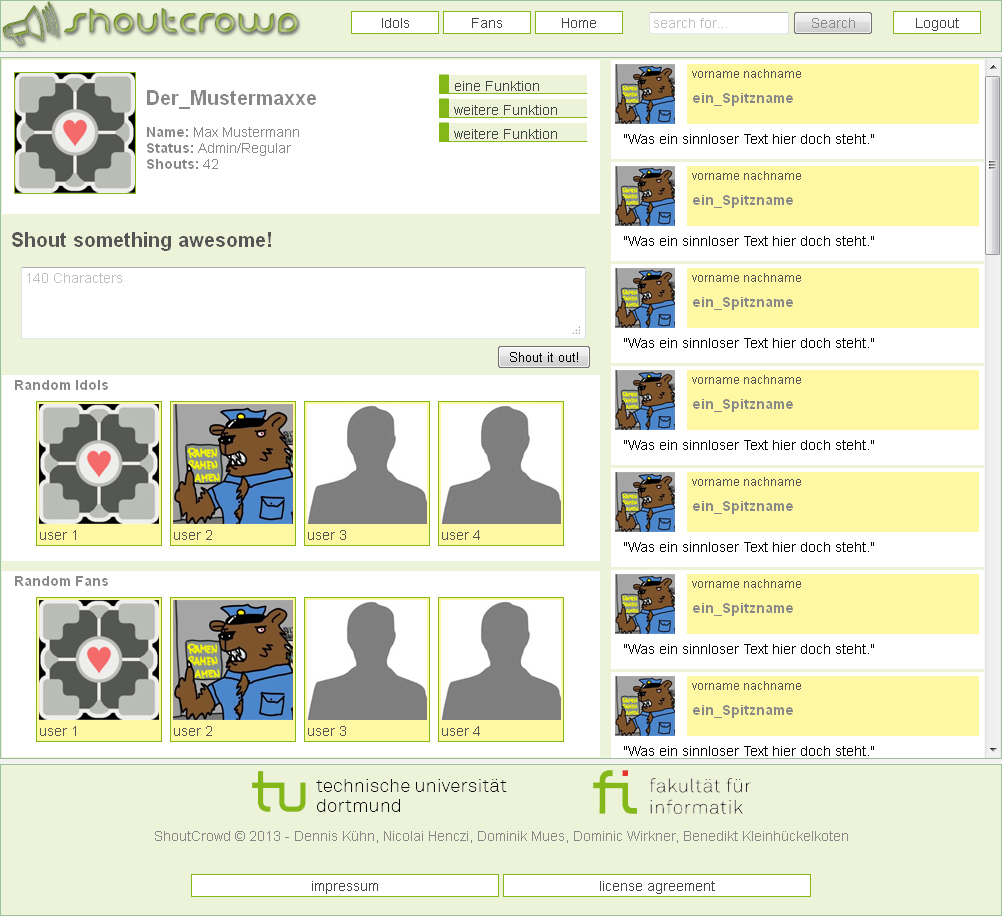
\includegraphics[width=0.9\textwidth]{first.jpg}
\caption{erstes Layout -- HTML mit statischen Inhalten per css optisch angepasst}
\end{center}
\end{figure}

\subsection*{Ladezeit}
Lange Wartezeiten zwischen einem Request und der Response resultieren oft daher, dass viele größere Bilder geladen werden müssen. Um das möglichst zu verhindern sind nur wenige Grafiken mit einer begrenzten Farbpalette (reduziert Dateigröße) in das Grundlayout eingeflossen. Enthalten sind ein eigenes Logo und die Logos der Universität und der Informatikfakultät, so wie ein Bild einer jubelnden Menge, welches zur Begrüßung angezeigt wird.

\subsection*{Haptik}
Die Wahrnehmung spielt nicht nur bei größeren Webprojekten mit vielen Funktionen eine große Rolle. Schon bei dem, doch recht beschaulichen, Projekt eines Twitter-Clons fallen viele Funktionen an, die Kontextspezifisch angeordnet werden müssen. So macht etwa ein "`Profil bearbeiten"'-Funktionen in einem Such Kontext keinen Sinn. Unsere Aufteilung beinhaltet eine Kopfnavigation mit den meistgenutzten Links (Idols, Fans, Home) und dem Logout-Button, so wie der Suche. Diese Seiten sollen von jedem Kotext aus erreichbar sein (*außer man ist nicht angemeldet; dann ist der logout-Button ein login-Button und die anderen Links führen auf die Startseite). Derart nebeneinander aufgelistete Funktionen in der Kopfzeile sind im Web 2.0 häufig zu finden und sollten deshalb vielen Nutzern bekannt vorkommen und einen intuitiven Umgang mit der Seite ermöglichen. Deutlich seltener genutzt werden Impressum, oder Lizenzvereinbarung. Diese Menüpunkte sind deshalb im Footer anzutreffen (welcher auch auf jeder Seite angezeigt wird). Kontextsensitiv sind Funktionen, wie beispielsweise "`Invite Fan"' oder "`Edit Profile"'. Derartige Aufrufe sind nur möglich in einer
 Auflistung von Usern (z.B. über die Suche) oder direkt auf der Profilseite dieses Benutzers. Idealerweise wäre der "`Edit Profile"'-Menüpunkt ein Unterpunkt von dem typischerweise in der Kopfzeile befindlichen "`Settings"'-Menüpunkt  gewesen. Da wir jedoch, zeitlich bedingt, auf die Implementierung weiterer Benutzereinstellungen verzichtet haben und die Kopfzeile sonst überladen wirken würde, wurde dieser Aspekt verworfen. Ebenfalls der Übersichtlichkeit und Gewohnheit der Benutzers geschuldet ist die Tatsache, dass jeder login/username nur in Verbindung mit seinem Avatar erscheint. Für den Fall, dass viele "`Shouts"' aufgelistet werden müssen, ist, um ein endloses Scrollen durch die Beiträge zu verhindern, eine Verteilung der Nachrichten auf mehrere Seiten implementiert (Pagination).  


\subsection*{Optische Wahrnehmung}
Die Optik in unserem Projekt war etwas, dass das wir ursprünglich vorhatten, zum Ende hin zu optimieren. Wie sich aber herausstellt, ist das anfänglich gewählte Layout durchaus mehr als ausreichend für den Projektumfang. Farblich wurde der Stil auf weiß für den Hintergrund, pastell gelblich bzw. grünlich für Rahmen, div-Hintergrundfarben und Links, schwarz für Schrift und rot für Fehlermeldungen und wichtige Hinweise festgesetzt. Durch die Rahmen, die die einzelnen Komponenten( in den div-Elementen enthalten) voneinander trennen, wirkt die Seite aufgeräumter und bekommt eine klarer definierte Struktur. Abweichend von der ursprünglich gewählten Ansicht, wird der Benutzer auf der Startseite von einem Bild einer jubelnden Menge "`begrüßt"' welches farblich und thematisch zum Rest des Projektes passt. Das Erscheinungsbild des Projektes wäre ausbaufähig zu einem kompletten Corporate Design.

\subsection*{Aufteilung der Komponenten/Pages}
Die Gestaltung und Verteilung der divs hat indirekte und direkte Auswirkungen auf Struktur der Komponenten und Pages. Nachdem es ein dreigliedriges Layout sein soll(Header, Content, Footer), macht es Sinn eine Komponente zu realisieren, die eben dieses Layout umsetzt. Innerhalb dieser Komponente wird die fest platzierte Komponente UserMenu (Header) und der Footer (nicht als Komponente, da der Inhalt des Footers nicht dynamisch ist), so wie eine body-Komponente, deren Inhalt von der aufrufenden Page bestimmt wird, angezeigt. Damit die Pages nicht zu unübersichtlich groß werden, sind einige Teile in Komponenten ausgelagert. Folgende Pages und Komponenten sind im Projekt enthalten:

\subsubsection*{Pages}
\begin{enumerate}
\item CreateAccount: Implementierung einer Benutzer Registrierung
\item EditProfile: Formular zum bearbeiten der angegebenen Benutzerdaten
\item Home: eigene Profilseite mit Profilinformationen und Shouts
\item Imprint: Obligatorisches Impressum (Platzhalter)
\item Index: Startseite, die zum Login oder zur Registrierung aufruft
\item Licence: Lizenzvereinbarung (nur Platzhalter für Rechtskräftigen Content) 
\item Login: Formular zum einloggen
\item Test: Testseite für die Entwickler (nicht für den normalen Benutzer gedacht)
\item ViewList: Auflistung von Usern durch Suche, Fans oder Idols
\item ViewProfile: wie Home, jedoch für fremde Profile
\item WipeAllData: Reset (für Angluin)
\end{enumerate}

\subsubsection*{Komponenten}
\begin{enumerate}
\item CreateMessage: Formular zur Eingabe von Shouts
\item Layout: (Erklärung siehe oben)
\item Pagination: Seitenzähler für Shouts
\item ProfileActions: Kontextabhängige Funktionsbuttons (Links)
\item ProfileDetails: selbsterklärend
\item ProfileListItem: Ansicht eines einzelnen Users in einer Auflistung
\item SingleMessage: Ansicht eines einzelnen Shouts
\item UserMenu: Die Kopfzeilen Navigation
\end{enumerate}

\subsection*{Abschließendes und Probleme}
Ziele unserer Gestaltung des Layouts sind eine einfache Umsetzung, ein komponentenunabhängiges Erscheinungsbild (zusammenpassend) und eine intuitive und leichte Bedienbarkeit. Zu letzterem ist zu sagen, dass für das Erreichen jeder Seite maximal drei Klicks notwendig sind und dem Benutzer entgegen gekommen wird, falls er beim Ausfüllen der Formulare etwas falsch gemacht hat. Komponentenunabhängigkeit ist durch eine nicht vorhandene statische Breitenzuweisung ebenfalls gewährleistet, was jedoch den Entwicklern die Möglichkeit bieten würde, Komponenten zu erstellen, die das Layout zerreißen würden. Dieses Problem ließe sich nur durch individuell angepasste Styles für jede Komponente verhindern. Die Umsetzung des Layouts und die spätere Einbindung in das Tapestry Projekt, erwies sich, bis auf kleinere Schwierigkeiten bei den Browserabhängigkeiten, als vergleichsweise einfach. Tapestry bietet allerdings keine (uns bekannte) Möglichkeit in CSS-Datein, Relative Pfade zu verwenden, wie dies in den TMLs möglich ist (Bsp:  \verb+<img src="${context:layout/images/logo.png}" alt="pic"/>+ ). Ausgehend von von den genannten Zielen und durchdachten Aspekten ist zu sagen, dass vieles mit einfachen Mitteln realisiert und dennoch nicht unterspezifiziert ist. 

